\documentclass{article}
\title{フーリエ解析入門 — 波を分解する数学}
\author{TeX 図書館}

\begin{document}

\section{この教科書のために — 波形のレシピ}

複雑な波(音楽・電気信号・株価の季節変動)も、\textbf{サイン波の重ね合わせ}として書ける——この 1800 年代の発見が、音楽圧縮(MP3)、画像圧縮(JPEG)、通信、音声認識の数学的基盤です。

フーリエ解析の世界観:\textbf{時間領域}(波が時間とともにどう揺れるか)と\textbf{周波数領域}(どんな周波数がどの強さで混ざっているか)は\textbf{同じ情報の 2 つの表現}であり、相互に翻訳できます。

\begin{quote}
\textbf{【例】}\ ピアノの「ド」の音。時間領域では複雑な波形ですが、周波数領域では「262 Hz が強く、その倍音が弱く」——\textbf{波形のレシピ}になります。音色の違いはレシピの違いです。
\end{quote}

\section{内積の直感 — 波を「測る」}

サイン波 \(\sin mx\) と \(\sin nx\) を区間 \([-\pi, \pi]\) で積分(= 関数の\textbf{内積})すると:
\[ \int_{-\pi}^{\pi} \sin mx \sin nx \, dx = 0 \quad (m \neq n) \]
——\textbf{異なる周波数のサイン波は直交する}のです。これは『大学数学入門』第 2 節のベクトルの内積(\(\boldsymbol{a} \cdot \boldsymbol{b} = 0\) で直交)の\textbf{関数版}です。

直交していると何が嬉しいか:\textbf{成分を他と混ぜずに独立に測れる}。ベクトル \(\boldsymbol{v}\) から x 成分を取り出すのが \(\boldsymbol{v} \cdot \boldsymbol{e}_x\) であるのと同じく、関数 \(f\) から「周波数 \(m\) の成分の大きさ」を取り出すのが
\[ b_m = \frac{1}{\pi} \int_{-\pi}^{\pi} f(x) \sin mx \, dx \]
です。\textbf{フーリエ級数の係数計算は「波との内積」}——この一貫した直感がすべてを支えます。

\begin{quote}
\textbf{【演習】}\ \(\int_{-\pi}^{\pi} \sin x \cos 2x \, dx = 0\) を「直交」の言葉で説明せよ。
\end{quote}

\textbf{解答の指針:}\ sin(奇関数)と cos(偶関数)の積は奇関数で、対称区間の積分は 0。周波数が違うだけでなく偶奇も違うため完全に直交します。

\section{フーリエ級数 — 周期関数のレシピ}

周期 \(2\pi\) の関数 \(f(x)\) は(収束の条件を満たせば):
\[ f(x) = \frac{a_0}{2} + \sum_{n=1}^{\infty} \left( a_n \cos nx + b_n \sin nx \right) \]
\[ a_n = \frac{1}{\pi} \int_{-\pi}^{\pi} f(x) \cos nx \, dx, \qquad b_n = \frac{1}{\pi} \int_{-\pi}^{\pi} f(x) \sin nx \, dx \]

\(a_n\): コサイン成分(偶の波)、\(b_n\): サイン成分(奇の波)。\textbf{偶関数なら \(b_n = 0\)、奇関数なら \(a_n = 0\)}——対象性がレシピを半分に省略します。

\begin{quote}
\textbf{【例:方形波】}\ \(-\pi < x < 0\) で \(-1\)、\(0 < x < \pi\) で \(+1\) という方形波。計算すると
\[ f(x) = \frac{4}{\pi} \left( \sin x + \frac{\sin 3x}{3} + \frac{\sin 5x}{5} + \cdots \right) \]
\textbf{奇数倍周波数のみ、振幅は \(1/3, 1/5\) と減衰}——角ばった波(急激な変化)を表すには高周波が必要で、その寄与は減衰していく。
\end{quote}

\begin{figure}[h]
\centering
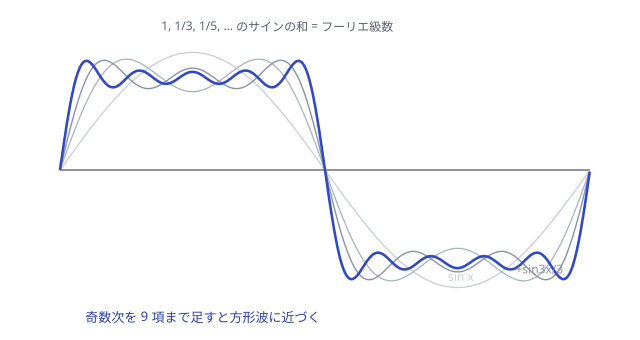
\includegraphics[width=0.85\textwidth]{figures/synthesis.svg}
\caption{奇数次のサイン波を重ねるほど方形波に近づく。}
\end{figure}

\begin{quote}
\textbf{【演習】}\ 方形波の \(n\) 項打ち切りで生じる誤差の「にぎり」(角の近くで振動する現象、ギブス現象)は、項数を増やしても角付近の高さは消えない。これは「無限和の極限」について何を示唆するか考察せよ。
\end{quote}

\textbf{解答の指針:}\ 各項は有限でも\textbf{無限和の収束の仕方}に注意が必要(一様収束しない)。連続でない関数のフーリエ級数は「点ごとの収束」しか保証しない——級数の理論の入口です。

\section{音の倍音 — 実例で見るレシピ}

楽器の音色は\textbf{倍音(高調波)の分布}で決まります。基音 \(f\) に対して:
\begin{itemize}
\item \textbf{フルート}: 奇数次の倍音が弱い(ほぼ純粋なサイン)
\item \textbf{バイオリン}: 幅広い倍音(角のない弓の摩擦でも成分が豊富)
\item \textbf{方形波状の音}: 奇数次のみ(\(1/3, 1/5\))——電子音のクラシックな「8bit 音」
\end{itemize}

イコライザーの「低音上げ・高音下げ」は、レシピの\textbf{特定行の強さを書き換える}操作です。MP3 圧縮は「人間の耳に聞こえにくい周波数成分(小さい係数)を捨てる」——フーリエ級数の\textbf{係数の刈り込み}です。

\begin{quote}
\textbf{【演習】}\ 「同じ音量の pure tone(純音)2 つ、293.7 Hz と 329.6 Hz を同時に鳴らす」と、うなり(周期的な強弱)が聞こえる。うなりの周期は差 35.9 Hz であることを、2 つのサインの和の式から説明せよ。
\end{quote}

\textbf{解答の指針:}\ 加法定理により \(\sin At + \sin Bt = 2\sin\frac{A+B}{2}t \cos\frac{A-B}{2}t\)。平均周波数の波が\textbf{差の半分の周波数}で揺れる(強弱の周期は \(2/35.9\) 秒)。

\section{離散フーリエ変換 — 計算機での実装}

実データは無限に続く連続関数ではなく\textbf{サンプル列}です。\(N\) 個のサンプルを周波数成分に分解するのが\textbf{離散フーリエ変換}( DFT ):
\[ X_k = \sum_{n=0}^{N-1} x_n\, e^{-2\pi i kn/N} \]
虚数単位 \(e^{i\theta} = \cos\theta + i\sin\theta\) は「サインとコサインを 1 つの式にまとめた」記法です(オイラーの公式)。

\begin{lstlisting}[language=Python]
import math

def dft(xs):
    N = len(xs)
    out = []
    for k in range(N):
        re = im = 0.0
        for n in range(N):
            ang = -2 * math.pi * k * n / N
            re += xs[n] * math.cos(ang)
            im += xs[n] * math.sin(ang)
        out.append(math.hypot(re, im))   # 振幅
    return out

# 「サイン波 + ノイズ」のスペクトル
xs = [math.sin(2*math.pi*n/8) + (random.random()-0.5)*0.3 for n in range(64)]
spec = dft(xs)
peak = max(range(1, 32), key=lambda k: spec[k])
print(peak)   # 8 が出る: 周期 8 サンプルの波を検出
\end{lstlisting}

\textbf{確認ポイント:} 周期 8 の波を混ぜたデータから、スペクトルのピークが「周波数ビン 8」に立つことを確認します。\textbf{信号の中の周期性が、スペクトルでは 1 本のピーク}として現れます。

\begin{quote}
\textbf{【演習】}\ DFT は \(N^2\) 回の計算が必要だが、FFT(高速フーリエ変換)は \(N \log N\) で済む。\(N = 10^6\) でどれだけ違うか概算せよ。
\end{quote}

\textbf{解答の指針:}\ \(10^{12}\) 対 \(2 \times 10^7\)、\textbf{5 万倍}。FFT がなければ現代の音声・画像・通信は計算時間的に不可能でした。

\section{スペクトルの読み方 — 応用の地形}

\begin{itemize}
\item \textbf{音声認識・音質調整}: スペクトルの形が音の正体
\item \textbf{JPEG 圧縮}: 画像を 2 次元フーリエ(正確にはコサイン変換)し、目立たない高周波成分を捨てる
\item \textbf{価格データ}: 季節変動・景気循環の周期をスペクトルから推定する(ただし非定常データには窓処理が必須——『時系列分析入門』参照)
\item \textbf{医療画像}(MRI): 磁気信号のフーリエ変換で断層像を再構成
\end{itemize}

\begin{quote}
\textbf{【演習】}\ 「12 か月周期の売上変動」と「1 週間周期の変動」が混ざったデータのスペクトルはどう見えるか予想し、どちらのピークが高くなるかを決める要因を述べよ。
\end{quote}

\textbf{解答の指針:}\ 2 本のピーク(年周期と週周期)。高さは\textbf{変動幅(振幅)の大きさ}で決まる。データ点数が少ないと 2 つのピークが混ざって見える(分解能 = 観測長さに反比例)。

\section{おわりに — 波で見る世界}

この教科書の骨格: 関数の内積(§2)が直交の概念を関数に拡張し、フーリエ級数(§3)が周期関数を周波数のレシピに翻訳し、倍音(§4)で音に実例を確かめ、DFT(§5)で計算機に載せ、スペクトル(§6)で応用の地形を見ました。

\textbf{「対象を分解して、その部品(周波数)の強さを見る」}——この発想は線形代数の固有値分解(『線形代数 応用編』)と\textbf{同じ構造}です(フーリエは「sin・cos という基底への分解」)。次の一歩は、離散コサイン変換(JPEG)、窓関数、そして『機械学習入門』でのスペクトル特徴の利用です。

\begin{quote}
\textbf{【総合演習】}
\begin{enumerate}
\item 偶関数のフーリエ級数で消える係数は?
\item 方形波のフーリエ級数で、\(x = \pi/2\) における最初の 3 項の値を計算し、方形波の値 +1 に近づくことを確かめよ。
\item FFT が \(N\log N\) で済む理由の発想(分割統治)を 1 文で述べよ。
\end{enumerate}
\end{quote}

\textbf{解答の指針:}\ 1. サイン成分 \(b_n\)。2. \(\frac{4}{\pi}(1 - \frac{1}{3} + \frac{1}{5}) = \frac{4}{\pi} \times \frac{13}{15} \approx 1.105\)。真値 1 に近い(オーバーシュートも見える)。3. 偶数番目と奇数番目に分解して小さい DFT 2 つに帰着させる(再帰)。

\end{document}
